\documentclass[class=jsarticle, crop=false, dvipdfmx, fleqn]{standalone}
%% preamble for Numerical-structure-analysis report

\input{/Users/User/Documents/Project/TeX/preamble/mypreamble}

%% titles
\title{統計的機械学習 レポート}
\author{37-196360 \quad 森田涼介}


%% setting for listings
\newtcbinputlisting[auto counter]{\reportlisting}[3][]{%
	listing file = {#3},
	listing options = {language=python, style=tcblatex, numbers=left, numberstyle=\tiny},
	listing only,
	breakable,
	toprule at break = 0mm,
	bottomrule at break = 0mm,
	left = 6mm,
	sharp corners,
	drop shadow,
	title = Listings \thetcbcounter : \texttt{#2},
	label = #1,
	}



%% title format
\usepackage{titlesec}
\titleformat{\section}{\LARGE}{宿題\thesection}{0zw}{}
\newcommand{\sectionbreak}{\clearpage}
\titleformat{\subsection}{\Large}{\Alph{subsection})}{0zw}{}

\begin{document}
\section{}

ガウスカーネルに対するカーネル密度推定法を行う。
バンド幅は尤度交差確認法によって決定する。


結果を以下の表\ref{tab:result}と図\ref{fig:result}に示した。
表\ref{tab:result}より,最も尤度の平均の大きいバンド幅は0.1となった。
なお,プログラムは\pageref{listing:assignment1}ページのListing \ref{listing:assignment1}に示した。


\begin{table}[H]
    \centering
    \caption{バンド幅とそれに対応するLCVの値}
    \begin{tabular}{lrrrr}
        \(h\) & 0.01 & 0.05 & 0.10 & 0.50 \\
        LCV & \(-6344\) & \(-4009\) & \(-3938\) & \(-4219\)
    \end{tabular}
    \label{tab:result}
\end{table}

\begin{figure}[H]
    \centering
    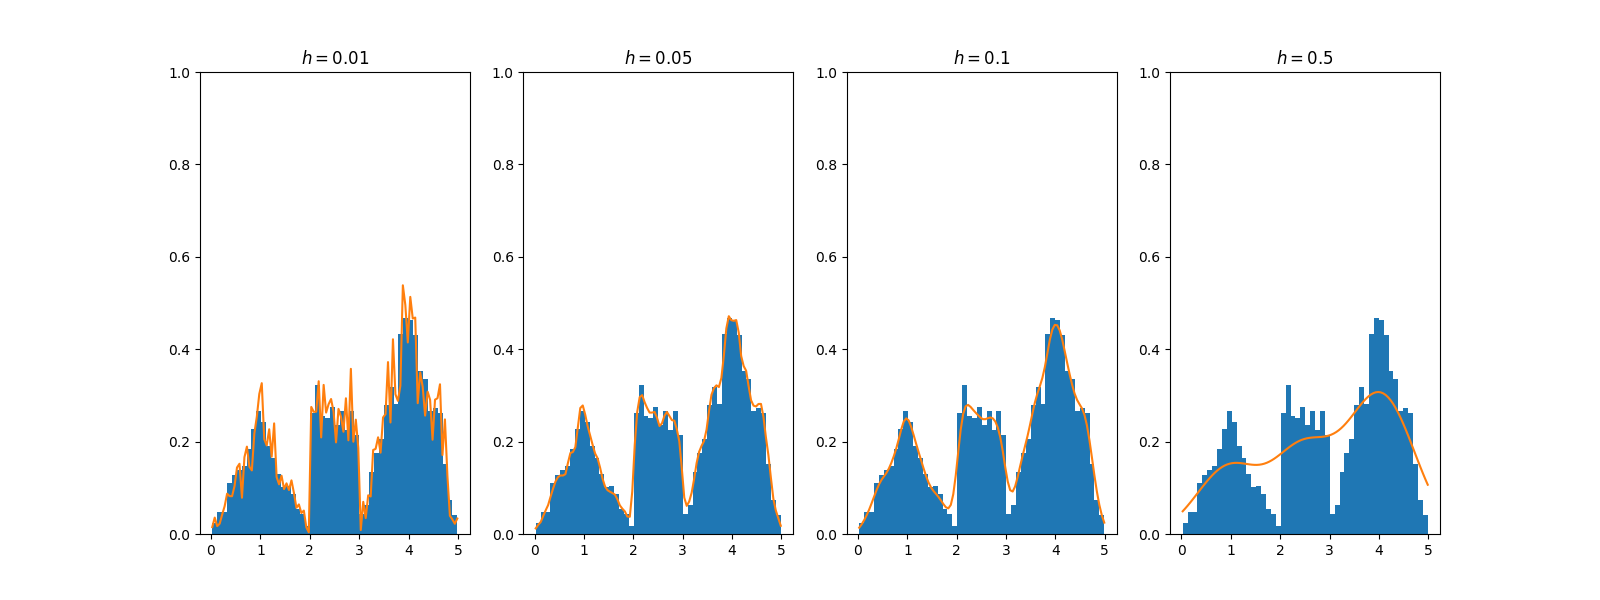
\includegraphics[clip, width=18cm]{../figures/assignment1_result_global}
    \caption{各バンド幅に対するヒストグラムと確率密度}
    \label{fig:result}
\end{figure}


\end{document}
